%% ============================================================
%% roberta_mamba_architecture.tex
%% Architecture diagram for roberta_mamba_freeze_init_4class
%% Compile with: xelatex roberta_mamba_architecture.tex
%% ============================================================
\documentclass[a4paper,12pt]{article}
\usepackage[margin=1.5cm]{geometry}
\usepackage{tikz}
\usetikzlibrary{arrows.meta, positioning, fit, backgrounds, calc}
\usepackage{amsmath, amssymb}
\usepackage{xcolor}
\usepackage{caption}
\usepackage{fontspec}
\usepackage{kotex}

\pagestyle{empty}

%% ---- Global TikZ styles ----
\tikzset{
  myarr/.style   = {-Stealth, line width=0.8pt},
  dasharr/.style = {-Stealth, line width=0.8pt, dashed},
  %% Box colour presets
  ibox/.style = {draw=gray!50,   fill=gray!15,   rounded corners=4pt, align=center, inner sep=5pt},
  ebox/.style = {draw=green!40,  fill=green!15,  rounded corners=4pt, align=center, inner sep=5pt},
  abox/.style = {draw=purple!50, fill=purple!20, rounded corners=4pt, align=center, inner sep=5pt, dashed},
  mbox/.style = {draw=orange!60, fill=orange!20, rounded corners=4pt, align=center, inner sep=5pt},
  hbox/.style = {draw=red!40,    fill=red!15,    rounded corners=4pt, align=center, inner sep=5pt},
  fbox/.style = {draw=blue!40,   fill=blue!15,   rounded corners=4pt, align=center, inner sep=5pt},
}

\begin{document}

%% ============================================================
%% FIGURE 1 — Local Encoder
%% ============================================================
\begin{figure}[ht]
\centering
\resizebox{\textwidth}{!}{%
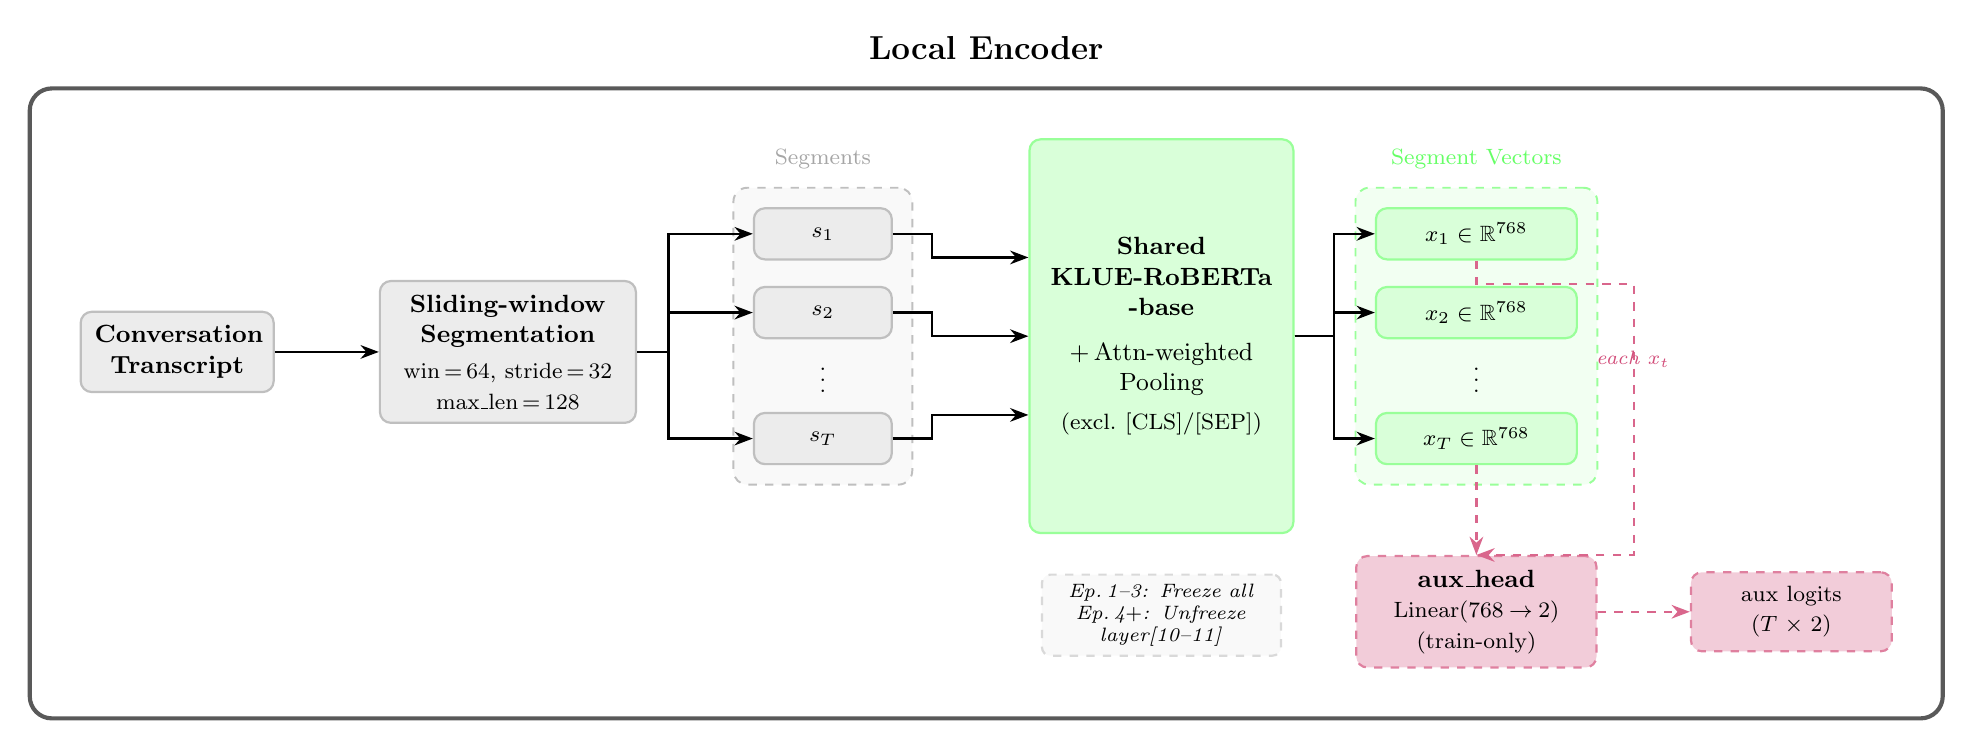
\begin{tikzpicture}[line width=0.8pt, >=Stealth, every node/.style={font=\small}]

%% ---- (1) Conversation Transcript ----
\node[ibox, text width=2.1cm] (transcript) at (0, 0) {
  \textbf{Conversation}\\
  \textbf{Transcript}
};

%% ---- (2) Sliding-window Segmentation ----
\node[ibox, text width=2.9cm] (sliding) at (4.2, 0) {
  \textbf{Sliding-window}\\
  \textbf{Segmentation}\\[2pt]
  {\footnotesize win\,=\,64, stride\,=\,32}\\
  {\footnotesize max\_len\,=\,128}
};

\draw[myarr] (transcript) -- (sliding);

%% ---- (3) Segments s_1 .. s_T ----
\node[ibox, text width=1.4cm, minimum height=0.65cm] (s1)    at (8.2,  1.5) {\footnotesize $s_1$};
\node[ibox, text width=1.4cm, minimum height=0.65cm] (s2)    at (8.2,  0.5) {\footnotesize $s_2$};
\node                                                 (sdots) at (8.2, -0.25) {\footnotesize $\vdots$};
\node[ibox, text width=1.4cm, minimum height=0.65cm] (sT)    at (8.2, -1.1) {\footnotesize $s_T$};

%% Arrows: sliding → segments (fan out to different heights on left side)
\draw[myarr] (sliding.east) -- ++(0.4,0) |- ($(s1.west)+(0,0)$);
\draw[myarr] (sliding.east) -- ++(0.4,0) |- ($(s2.west)+(0,0)$);
\draw[myarr] (sliding.east) -- ++(0.4,0) |- ($(sT.west)+(0,0)$);

%% ---- (4) Shared KLUE-RoBERTa-base Encoder ----
\node[ebox, text width=3.0cm, minimum height=5.0cm] (encoder) at (12.5, 0.2) {
  \textbf{Shared}\\
  \textbf{KLUE-RoBERTa}\\
  \textbf{-base}\\[5pt]
  {\small $+$\,Attn-weighted}\\
  {\small Pooling}\\[3pt]
  {\footnotesize (excl.\ [CLS]/[SEP])}
};

%% Arrows: segments → encoder (enter at different y-offsets for clarity)
\draw[myarr] (s1.east) -- ++(0.5,0) |- ($(encoder.west)+(0, 1.0)$);
\draw[myarr] (s2.east) -- ++(0.5,0) |- ($(encoder.west)+(0, 0.0)$);
\draw[myarr] (sT.east) -- ++(0.5,0) |- ($(encoder.west)+(0,-1.0)$);

%% Freeze annotation (below encoder)
\node[draw=gray!30, fill=gray!5, dashed, rounded corners=3pt,
      font=\scriptsize, text width=2.8cm, align=center,
      below=0.5cm of encoder] (freeze) {
  \textit{Ep.\,1--3: Freeze all}\\
  \textit{Ep.\,4$+$: Unfreeze}\\
  \textit{layer[10--11]}
};

%% ---- (5) Output segment vectors x_1 .. x_T ----
\node[ebox, text width=2.2cm, minimum height=0.65cm] (x1)    at (16.5,  1.5) {\footnotesize $x_1\!\in\!\mathbb{R}^{768}$};
\node[ebox, text width=2.2cm, minimum height=0.65cm] (x2)    at (16.5,  0.5) {\footnotesize $x_2\!\in\!\mathbb{R}^{768}$};
\node                                                 (xdots) at (16.5, -0.25) {\footnotesize $\vdots$};
\node[ebox, text width=2.2cm, minimum height=0.65cm] (xT)    at (16.5, -1.1) {\footnotesize $x_T\!\in\!\mathbb{R}^{768}$};

%% Arrows: encoder → output vectors
\draw[myarr] (encoder.east) -- ++(0.5,0) |- ($(x1.west)+(0,0)$);
\draw[myarr] (encoder.east) -- ++(0.5,0) |- ($(x2.west)+(0,0)$);
\draw[myarr] (encoder.east) -- ++(0.5,0) |- ($(xT.west)+(0,0)$);

%% ---- (6) Aux head — train-only (dashed purple) ----
\node[abox, text width=2.7cm] (auxhead) at (16.5, -3.3) {
  \textbf{aux\_head}\\
  {\footnotesize Linear($768\!\to\!2$)}\\
  {\footnotesize (train-only)}
};
\node[abox, text width=2.2cm] (auxlogits) at (20.5, -3.3) {
  {\footnotesize aux logits}\\
  {\footnotesize $(T \times 2)$}
};

%% All x_t feed aux_head; show representative arrows from x1 & xT
\draw[dasharr, draw=purple!60]
  (xT.south) -- ++(0,-0.55) -| (auxhead.north);
\draw[dasharr, draw=purple!60]
  (x1.south) -- ++(0,-0.3) -- ++(2.0,0) |- (auxhead.north);
\draw[dasharr, draw=purple!60] (auxhead) -- (auxlogits);

%% Annotation near dashed arrows
\node[font=\scriptsize, text=purple!70, below right=0.02cm and 0.1cm of x2]
  {\textit{each $x_t$}};

%% ---- Background decorations ----
\begin{pgfonlayer}{background}
  %% Outer figure bounding box
  \node[draw=black!65, line width=1.5pt, rounded corners=8pt, fill=none,
        fit=(transcript)(sliding)(s1)(sT)(encoder)(freeze)(x1)(xT)(auxhead)(auxlogits),
        inner sep=18pt] (fig1outer) {};

  %% Segment group box
  \node[draw=gray!50, dashed, line width=0.7pt, fill=gray!5,
        rounded corners=5pt,
        fit=(s1)(sT)(sdots), inner sep=7pt] (seggrp) {};

  %% Segment-vector group box
  \node[draw=green!40, dashed, line width=0.7pt, fill=green!5,
        rounded corners=5pt,
        fit=(x1)(xT)(xdots), inner sep=7pt] (xvecgrp) {};
\end{pgfonlayer}

%% Group / figure labels (foreground so they are not hidden by fills)
\node[above=3pt of seggrp,  font=\footnotesize, text=gray!70]  {Segments};
\node[above=3pt of xvecgrp, font=\footnotesize, text=green!60] {Segment Vectors};
\node[above=6pt of fig1outer, font=\large\bfseries] {Local Encoder};

\end{tikzpicture}%
}%
\caption{Local Encoder: KLUE-RoBERTa-base encodes each segment into a 768-dim vector via attention-weighted pooling.}
\label{fig:local-encoder}
\end{figure}

\clearpage

%% ============================================================
%% FIGURE 2 — Global Context Model
%% ============================================================
\begin{figure}[ht]
\centering
\resizebox{\textwidth}{!}{%
\begin{tikzpicture}[line width=0.8pt, >=Stealth, every node/.style={font=\small}]

%% ---- (1) Input sequence X ----
\node[ibox, text width=2.6cm] (inputX) at (0, 0) {
  $X\!=\![x_1,\ldots,x_T]$\\
  {\footnotesize $\in\mathbb{R}^{T\times768}$}\\
  {\scriptsize (from Fig.\,1)}
};

%% ---- (2) 2-layer Mamba SSM Stack ----
\node[mbox, text width=2.9cm, minimum height=4.2cm] (mamba) at (4.8, 0) {
  \textbf{2-layer Mamba}\\
  \textbf{SSM Stack}\\[5pt]
  {\footnotesize $D_{\mathrm{model}}=768$}\\
  {\footnotesize $D_{\mathrm{state}}=16$}\\
  {\footnotesize $D_{\mathrm{conv}}=4$}\\
  {\footnotesize expand$\;=2$}\\[3pt]
  {\footnotesize $L=2$}
};

\draw[myarr] (inputX) -- (mamba);

%% ---- (3) Hidden states h_1 .. h_T ----
\node[mbox, text width=1.7cm, minimum height=0.65cm] (h1)    at (9.5,  1.5) {\footnotesize $h_1$};
\node[mbox, text width=1.7cm, minimum height=0.65cm] (h2)    at (9.5,  0.5) {\footnotesize $h_2$};
\node                                                 (hdots) at (9.5, -0.25) {\footnotesize $\vdots$};
\node[mbox, text width=1.7cm, minimum height=0.65cm] (hT)    at (9.5, -1.1) {\footnotesize $h_T$};

\draw[myarr] (mamba.east) -- ++(0.4,0) |- ($(h1.west)+(0,0)$);
\draw[myarr] (mamba.east) -- ++(0.4,0) |- ($(h2.west)+(0,0)$);
\draw[myarr] (mamba.east) -- ++(0.4,0) |- ($(hT.west)+(0,0)$);

%% ---- (4) Last Valid State ----
\node[mbox, text width=2.6cm] (laststate) at (13.3, -1.1) {
  \textbf{Last Valid}\\
  \textbf{State}\;$h_T$\\
  {\footnotesize idx:\;$T\!-\!1$}
};

\draw[myarr] (hT.east) -- (laststate.west);
%% Indicate h_1..h_{T-1} are not forwarded
\draw[myarr, draw=gray!30]
  (h1.east) -- ++(0.25,0) node[right, font=\scriptsize, text=gray!50] {};

%% ---- (5) HierarchicalHead — shared pre-processing ----
\node[hbox, text width=3.0cm, minimum height=4.8cm] (shared) at (17.5, -1.1) {
  \textbf{Hierarchical}\\
  \textbf{Head}\\[6pt]
  {\footnotesize LayerNorm}\\
  {\footnotesize $\downarrow$}\\
  {\footnotesize Linear($768\!\to\!64$)}\\
  {\footnotesize $\downarrow$}\\
  {\footnotesize GELU}\\
  {\footnotesize $\downarrow$}\\
  {\footnotesize Dropout(0.1)}
};

\draw[myarr] (laststate.east) -- (shared.west);

%% ---- (6) Three branch heads ----
\node[hbox, text width=2.9cm] (superhead)    at (22.2,  2.0) {
  \textbf{superclass\_head}\\
  {\footnotesize Linear($64\!\to\!2$)}
};
\node[hbox, text width=2.9cm] (normalhead)   at (22.2, -1.1) {
  \textbf{normal\_head}\\
  {\footnotesize Linear($64\!\to\!2$)}
};
\node[hbox, text width=2.9cm] (phishinghead) at (22.2, -4.2) {
  \textbf{phishing\_head}\\
  {\footnotesize Linear($64\!\to\!2$)}
};

%% Shared → branch heads
\draw[myarr] (shared.east) -- ++(0.3,0) |- (superhead.west);
\draw[myarr] (shared.east) -- ++(0.3,0) |- (normalhead.west);
\draw[myarr] (shared.east) -- ++(0.3,0) |- (phishinghead.west);

%% ---- (7) Logits ----
\node[hbox, text width=3.0cm] (superlogits)    at (26.7,  2.0) {
  \textbf{super\_logits}\\
  {\footnotesize Normal / Phishing}
};
\node[hbox, text width=3.0cm] (normallogits)   at (26.7, -1.1) {
  \textbf{normal\_logits}\\
  {\footnotesize 상담 대화 /}\\
  {\footnotesize 일상 대화}
};
\node[hbox, text width=3.0cm] (phishinglogits) at (26.7, -4.2) {
  \textbf{phishing\_logits}\\
  {\footnotesize 대출 사기형 /}\\
  {\footnotesize 수사기관 사칭형}
};

\draw[myarr] (superhead)    -- (superlogits);
\draw[myarr] (normalhead)   -- (normallogits);
\draw[myarr] (phishinghead) -- (phishinglogits);

%% ---- (8) Hierarchical Fusion ----
\node[fbox, text width=3.2cm] (fusion) at (31.2, -1.1) {
  \textbf{Hierarchical}\\
  \textbf{Fusion}\\[5pt]
  {\footnotesize $P(y)=P(\mathrm{super})$}\\[1pt]
  {\footnotesize $\otimes\;P(\mathrm{sub}\mid\mathrm{super})$}\\[3pt]
  {\scriptsize softmax(super)}\\
  {\scriptsize $\otimes$ [softmax(normal),}\\
  {\scriptsize softmax(phishing)]}
};

%% Logits → Fusion
\draw[myarr] (superlogits.east)    -- ++(0.3,0) |- (fusion.north);
\draw[myarr] (normallogits.east)   -- ++(0.3,0) -- (fusion.west);
\draw[myarr] (phishinglogits.east) -- ++(0.3,0) |- (fusion.south);

%% ---- (9) Final 4-class Prediction ----
\node[fbox, text width=3.0cm] (output) at (35.6, -1.1) {
  \textbf{Final 4-class}\\
  \textbf{Prediction}\\[5pt]
  {\footnotesize 상담 대화}\\
  {\footnotesize 일상 대화}\\
  {\footnotesize 대출 사기형}\\
  {\footnotesize 수사기관 사칭형}
};

\draw[myarr] (fusion) -- (output);

%% ---- Background decorations ----
\begin{pgfonlayer}{background}
  %% Outer figure bounding box
  \node[draw=black!65, line width=1.5pt, rounded corners=8pt, fill=none,
        fit=(inputX)(mamba)(h1)(hT)(laststate)(shared)
            (superhead)(phishinghead)(superlogits)(phishinglogits)
            (fusion)(output),
        inner sep=18pt] (fig2outer) {};

  %% Hidden-states group box
  \node[draw=orange!60, dashed, line width=0.7pt, fill=orange!5,
        rounded corners=5pt,
        fit=(h1)(hT)(hdots), inner sep=7pt] (hgrp) {};
\end{pgfonlayer}

%% Labels (foreground)
\node[above=3pt of hgrp,     font=\footnotesize, text=orange!70] {Hidden States};
\node[above=6pt of fig2outer, font=\large\bfseries]              {Global Context Model};

\end{tikzpicture}%
}%
\caption{Global Context Model: Mamba SSM models temporal belief over segments; hierarchical heads produce 4-class output.}
\label{fig:global-context}
\end{figure}

\end{document}
